\documentclass{book}
\usepackage[a4paper,top=2.5cm,bottom=2.5cm,left=2.5cm,right=2.5cm]{geometry}
\usepackage{makeidx}
\usepackage{natbib}
\usepackage{graphicx}
\usepackage{multicol}
\usepackage{float}
\usepackage{listings}
\usepackage{color}
\usepackage{ifthen}
\usepackage[table]{xcolor}
\usepackage{textcomp}
\usepackage{alltt}
\usepackage{ifpdf}
\ifpdf
\usepackage[pdftex,
            pagebackref=true,
            colorlinks=true,
            linkcolor=blue,
            unicode
           ]{hyperref}
\else
\usepackage[ps2pdf,
            pagebackref=true,
            colorlinks=true,
            linkcolor=blue,
            unicode
           ]{hyperref}
\usepackage{pspicture}
\fi
\usepackage[utf8]{inputenc}
\usepackage[T2A]{fontenc}
\usepackage[russian]{babel}

\usepackage{mathptmx}
\usepackage[scaled=.90]{helvet}
\usepackage{courier}
\usepackage{sectsty}
\usepackage{amssymb}
\usepackage[titles]{tocloft}
\usepackage{doxygen}
\lstset{language=C++,inputencoding=utf8,basicstyle=\footnotesize,breaklines=true,breakatwhitespace=true,tabsize=4,numbers=left }
\makeindex
\setcounter{tocdepth}{3}
\renewcommand{\footrulewidth}{0.4pt}
\renewcommand{\familydefault}{\sfdefault}
\hfuzz=15pt
\setlength{\emergencystretch}{15pt}
\hbadness=750
\tolerance=750
\begin{document}
\hypersetup{pageanchor=false,citecolor=blue}
\begin{titlepage}
\vspace*{7cm}
\begin{center}
{\Large T2\-C Manager }\\
\vspace*{1cm}
{\large Создано системой Doxygen 1.8.3.1}\\
\vspace*{0.5cm}
{\small Сб 20 Апр 2013 00:48:27}\\
\end{center}
\end{titlepage}
\clearemptydoublepage
\pagenumbering{roman}
\tableofcontents
\clearemptydoublepage
\pagenumbering{arabic}
\hypersetup{pageanchor=true,citecolor=blue}
\chapter{Иерархический список классов}
\section{Иерархия классов}
Иерархия классов.\begin{DoxyCompactList}
\item Plugin\begin{DoxyCompactList}
\item \contentsline{section}{T2\-C\-Factory}{\pageref{class_t2_c_factory}}{}
\end{DoxyCompactList}
\item \contentsline{section}{P\-V}{\pageref{struct_p_v}}{}
\item Q\-Object\begin{DoxyCompactList}
\item \contentsline{section}{P\-V\-Listener}{\pageref{class_p_v_listener}}{}
\item \contentsline{section}{T2\-C\-Manager}{\pageref{class_t2_c_manager}}{}
\end{DoxyCompactList}
\item \contentsline{section}{Token\-List}{\pageref{class_token_list}}{}
\end{DoxyCompactList}

\chapter{Алфавитный указатель классов}
\section{Классы}
Классы с их кратким описанием.\begin{DoxyCompactList}
\item\contentsline{section}{\hyperlink{struct_p_v}{P\-V} \\*Структура, хранящая информацию о процессной переменной }{\pageref{struct_p_v}}{}
\item\contentsline{section}{\hyperlink{class_p_v_listener}{P\-V\-Listener} \\*\hyperlink{class_p_v_listener}{P\-V\-Listener} выдаёт сигнал value\-Updated при изменении значения связанной процессной переменной }{\pageref{class_p_v_listener}}{}
\item\contentsline{section}{\hyperlink{class_t2_c_factory}{T2\-C\-Factory} }{\pageref{class_t2_c_factory}}{}
\item\contentsline{section}{\hyperlink{class_t2_c_manager}{T2\-C\-Manager} \\*\hyperlink{class_t2_c_manager}{T2\-C\-Manager} -\/ модуль для работы с интерфейсом T2\-C }{\pageref{class_t2_c_manager}}{}
\item\contentsline{section}{\hyperlink{class_token_list}{Token\-List} }{\pageref{class_token_list}}{}
\end{DoxyCompactList}

\chapter{Классы}
\hypertarget{struct_p_v}{\section{Структура P\-V}
\label{struct_p_v}\index{P\-V@{P\-V}}
}


Структура, хранящая информацию о процессной переменной  




{\ttfamily \#include $<$t2c.\-h$>$}

\subsection*{Открытые атрибуты}
\begin{DoxyCompactItemize}
\item 
\hypertarget{struct_p_v_abf7a2b104815f063f098b3f12cb5efb4}{Q\-Date\-Time \hyperlink{struct_p_v_abf7a2b104815f063f098b3f12cb5efb4}{time}}\label{struct_p_v_abf7a2b104815f063f098b3f12cb5efb4}

\begin{DoxyCompactList}\small\item\em Метка времени \end{DoxyCompactList}\item 
\hypertarget{struct_p_v_a1e4608363410a01ca0b73d61fb898656}{Q\-Variant \hyperlink{struct_p_v_a1e4608363410a01ca0b73d61fb898656}{value}}\label{struct_p_v_a1e4608363410a01ca0b73d61fb898656}

\begin{DoxyCompactList}\small\item\em Значение \end{DoxyCompactList}\item 
\hypertarget{struct_p_v_a02551777c1773cd8d67195be4ba18653}{quint16 \hyperlink{struct_p_v_a02551777c1773cd8d67195be4ba18653}{status}}\label{struct_p_v_a02551777c1773cd8d67195be4ba18653}

\begin{DoxyCompactList}\small\item\em Статус \end{DoxyCompactList}\item 
\hypertarget{struct_p_v_a8929ed79170ed8f87817646de10799fe}{Q\-Byte\-Array \hyperlink{struct_p_v_a8929ed79170ed8f87817646de10799fe}{i\-Type}}\label{struct_p_v_a8929ed79170ed8f87817646de10799fe}

\begin{DoxyCompactList}\small\item\em Текстовое обозначение типа данных в Control\-Star. \end{DoxyCompactList}\item 
bool \hyperlink{struct_p_v_a865f200b8c4ea2cb89894e7133245bb7}{subscribed}
\begin{DoxyCompactList}\small\item\em Флаг подписки. \end{DoxyCompactList}\item 
bool \hyperlink{struct_p_v_ab53638c0e66c5b2b86cea564f02e2947}{changed}
\begin{DoxyCompactList}\small\item\em Флаг изменения. \end{DoxyCompactList}\item 
\hypertarget{struct_p_v_ab0718ffead2b27c26125e83475de016b}{\hyperlink{class_p_v_listener}{P\-V\-Listener} $\ast$ \hyperlink{struct_p_v_ab0718ffead2b27c26125e83475de016b}{listener}}\label{struct_p_v_ab0718ffead2b27c26125e83475de016b}

\begin{DoxyCompactList}\small\item\em Указатель на объект listener. \end{DoxyCompactList}\end{DoxyCompactItemize}


\subsection{Подробное описание}
Структура, хранящая информацию о процессной переменной 

\subsection{Данные класса}
\hypertarget{struct_p_v_ab53638c0e66c5b2b86cea564f02e2947}{\index{P\-V@{P\-V}!changed@{changed}}
\index{changed@{changed}!PV@{P\-V}}
\subsubsection[{changed}]{\setlength{\rightskip}{0pt plus 5cm}bool P\-V\-::changed}}\label{struct_p_v_ab53638c0e66c5b2b86cea564f02e2947}


Флаг изменения. 

Установлен, если значение кем-\/то изменено, и необходима синхронизация со S\-C\-A\-D\-A. \hypertarget{struct_p_v_a865f200b8c4ea2cb89894e7133245bb7}{\index{P\-V@{P\-V}!subscribed@{subscribed}}
\index{subscribed@{subscribed}!PV@{P\-V}}
\subsubsection[{subscribed}]{\setlength{\rightskip}{0pt plus 5cm}bool P\-V\-::subscribed}}\label{struct_p_v_a865f200b8c4ea2cb89894e7133245bb7}


Флаг подписки. 

Установлен, если значение этой ПП обновляется автоматически. 

Объявления и описания членов структуры находятся в файле\-:\begin{DoxyCompactItemize}
\item 
t2c.\-h\end{DoxyCompactItemize}

\hypertarget{class_p_v_listener}{\section{Класс P\-V\-Listener}
\label{class_p_v_listener}\index{P\-V\-Listener@{P\-V\-Listener}}
}


\hyperlink{class_p_v_listener}{P\-V\-Listener} выдаёт сигнал value\-Updated при изменении значения связанной процессной переменной  




{\ttfamily \#include $<$t2c.\-h$>$}

Граф наследования\-:P\-V\-Listener\-:\begin{figure}[H]
\begin{center}
\leavevmode
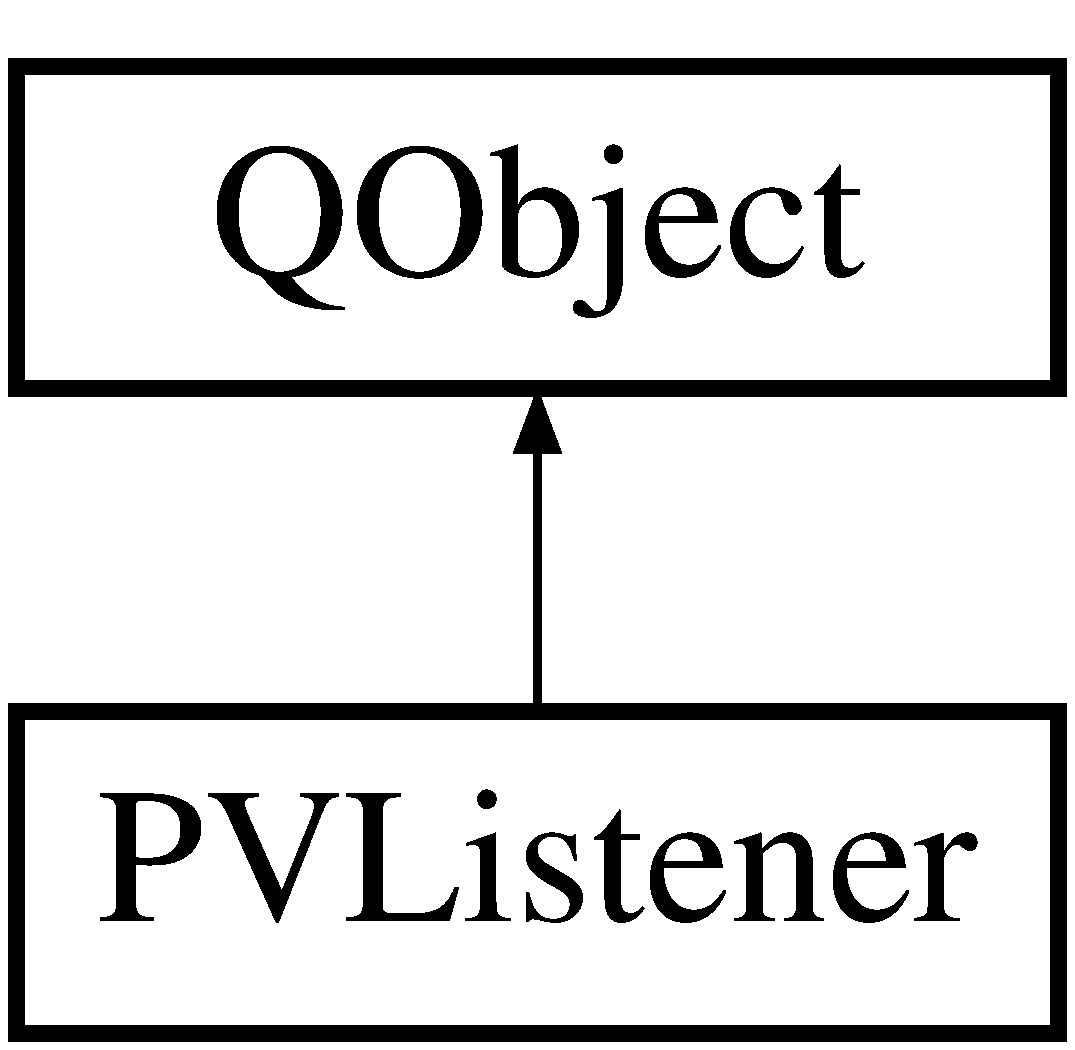
\includegraphics[height=2.000000cm]{class_p_v_listener}
\end{center}
\end{figure}
\subsection*{Открытые слоты}
\begin{DoxyCompactItemize}
\item 
\hypertarget{class_p_v_listener_abe135090bdd633ebceae1f45c092257e}{void {\bfseries on\-Update} (int idf)}\label{class_p_v_listener_abe135090bdd633ebceae1f45c092257e}

\end{DoxyCompactItemize}
\subsection*{Сигналы}
\begin{DoxyCompactItemize}
\item 
\hypertarget{class_p_v_listener_a35b4710a384a4fce528471c257a1bae6}{void {\bfseries value\-Updated} (int idf)}\label{class_p_v_listener_a35b4710a384a4fce528471c257a1bae6}

\end{DoxyCompactItemize}
\subsection*{Открытые члены}
\begin{DoxyCompactItemize}
\item 
\hypertarget{class_p_v_listener_ab9fd3bf9f09a8a47316c039d9244d96a}{{\bfseries P\-V\-Listener} (int pvcount)}\label{class_p_v_listener_ab9fd3bf9f09a8a47316c039d9244d96a}

\item 
\hypertarget{class_p_v_listener_a96dacdc1e1295bb889d64737fe8efa39}{bool {\bfseries deref} ()}\label{class_p_v_listener_a96dacdc1e1295bb889d64737fe8efa39}

\end{DoxyCompactItemize}


\subsection{Подробное описание}
\hyperlink{class_p_v_listener}{P\-V\-Listener} выдаёт сигнал value\-Updated при изменении значения связанной процессной переменной 

Объявления и описания членов классов находятся в файлах\-:\begin{DoxyCompactItemize}
\item 
t2c.\-h\item 
moc\-\_\-t2c.\-cpp\end{DoxyCompactItemize}

\hypertarget{class_t2_c_factory}{\section{Класс T2\-C\-Factory}
\label{class_t2_c_factory}\index{T2\-C\-Factory@{T2\-C\-Factory}}
}
Граф наследования\-:T2\-C\-Factory\-:\begin{figure}[H]
\begin{center}
\leavevmode
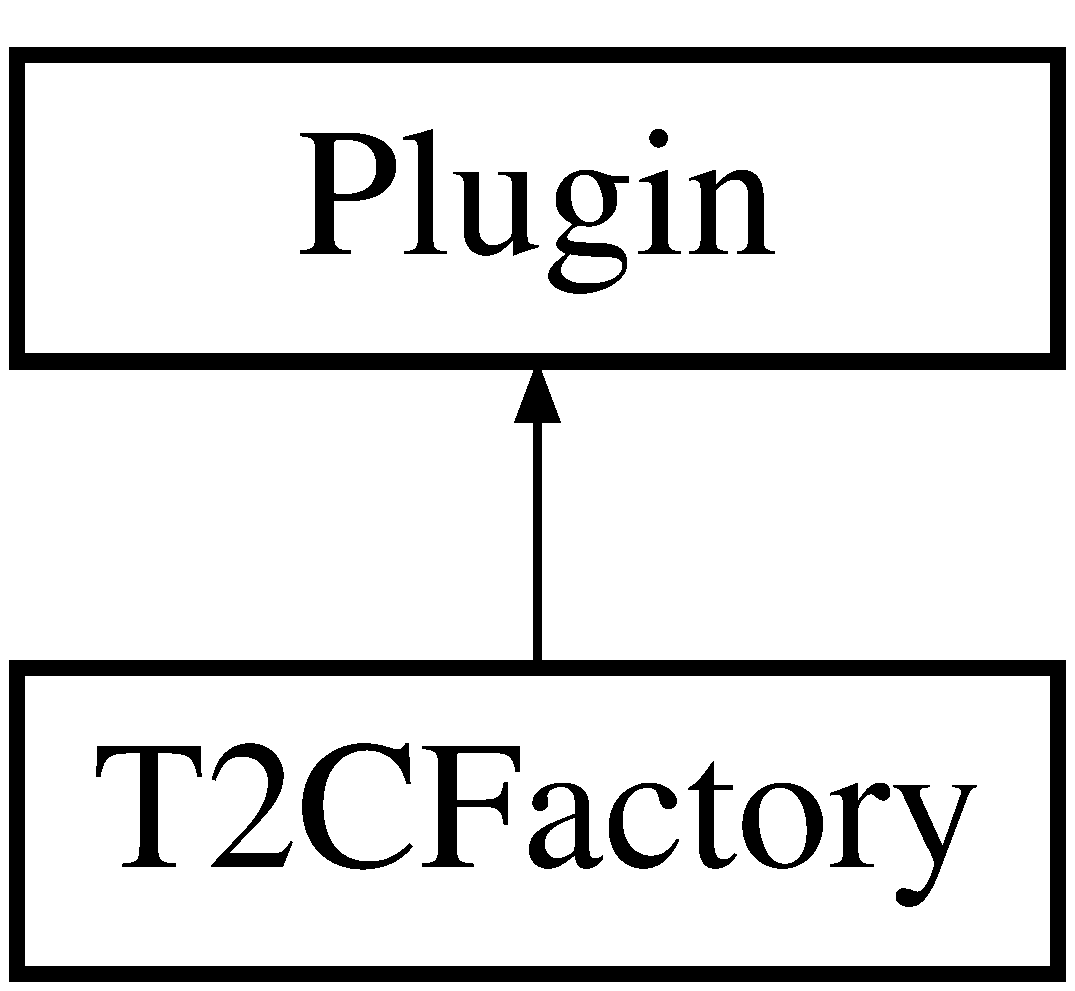
\includegraphics[height=2.000000cm]{class_t2_c_factory}
\end{center}
\end{figure}
\subsection*{Открытые члены}
\begin{DoxyCompactItemize}
\item 
\hypertarget{class_t2_c_factory_ab411a46a7147ee8d1130697aeca2eb29}{Q\-Object $\ast$ {\bfseries new\-Instance} ()}\label{class_t2_c_factory_ab411a46a7147ee8d1130697aeca2eb29}

\item 
\hypertarget{class_t2_c_factory_a51a7dac626d2972dd5729f9a0d49f756}{int {\bfseries init} (Q\-Object $\ast$core)}\label{class_t2_c_factory_a51a7dac626d2972dd5729f9a0d49f756}

\item 
\hypertarget{class_t2_c_factory_aabbd4502d962a7c888c0531eac257790}{Q\-Variant\-Hash {\bfseries get\-Info} ()}\label{class_t2_c_factory_aabbd4502d962a7c888c0531eac257790}

\end{DoxyCompactItemize}


Объявления и описания членов классов находятся в файлах\-:\begin{DoxyCompactItemize}
\item 
t2c.\-h\item 
t2c.\-cpp\end{DoxyCompactItemize}

\hypertarget{class_t2_c_manager}{\section{Класс T2\-C\-Manager}
\label{class_t2_c_manager}\index{T2\-C\-Manager@{T2\-C\-Manager}}
}


\hyperlink{class_t2_c_manager}{T2\-C\-Manager} -\/ модуль для работы с интерфейсом T2\-C.  




{\ttfamily \#include $<$t2c.\-h$>$}

Граф наследования\-:T2\-C\-Manager\-:\begin{figure}[H]
\begin{center}
\leavevmode
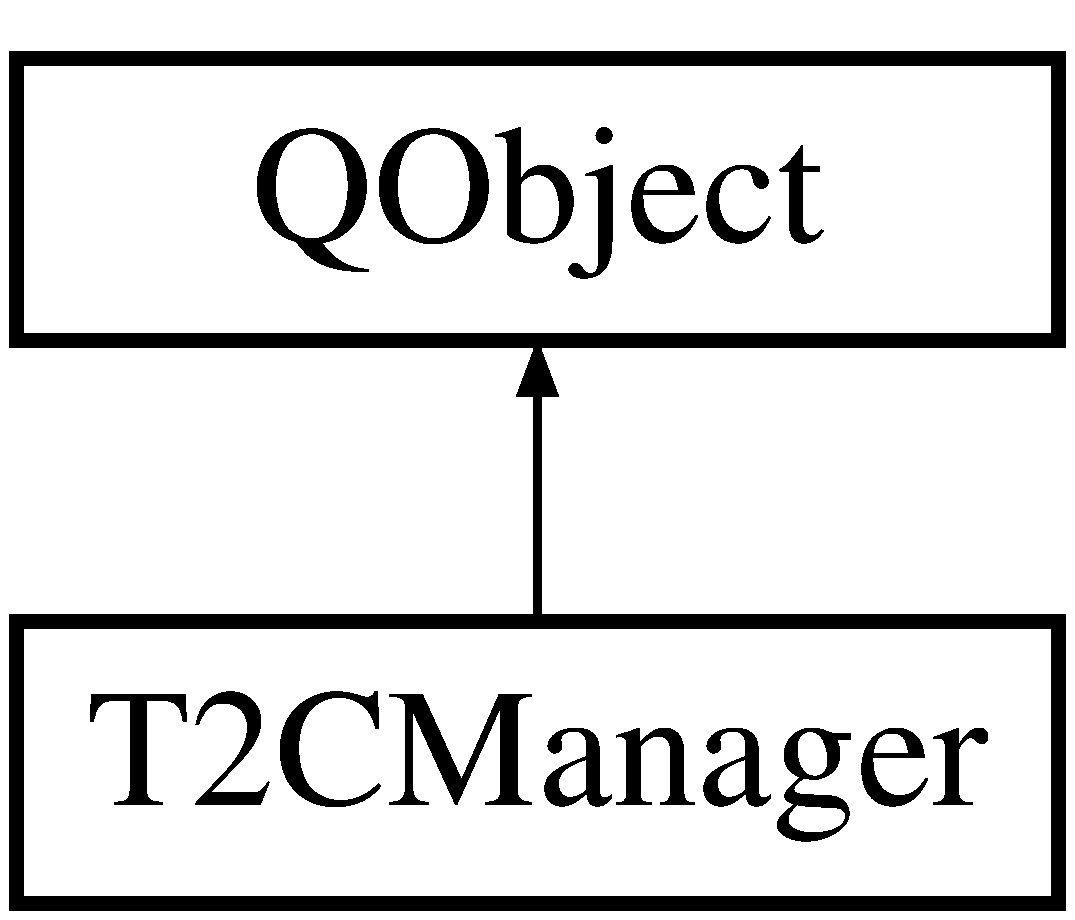
\includegraphics[height=2.000000cm]{class_t2_c_manager}
\end{center}
\end{figure}
\subsection*{Открытые слоты}
\begin{DoxyCompactItemize}
\item 
void \hyperlink{class_t2_c_manager_a43508413b4a7d90407e14f1d5005a0b5}{set\-Encoding} (Q\-String arg)
\begin{DoxyCompactList}\small\item\em Устанавливает кодировку для обмена с T2\-C. \end{DoxyCompactList}\item 
void \hyperlink{class_t2_c_manager_aa696512a3ebc03c497629ca19f903cad}{set\-Immediate} (bool arg)
\begin{DoxyCompactList}\small\item\em Управляет режимом немедленной записи изменений. \end{DoxyCompactList}\item 
void \hyperlink{class_t2_c_manager_a1d3657acdeeacde9e155b6924211eff1}{set\-Raw\-Mode} (bool arg)
\begin{DoxyCompactList}\small\item\em Управляет «сырым» режимом. \end{DoxyCompactList}\item 
\hyperlink{struct_p_v}{P\-V} \hyperlink{class_t2_c_manager_a015b9e2a04b88549b7c48e84e66a8a51}{get\-P\-V} (int idf, bool force\-Cached=true)
\begin{DoxyCompactList}\small\item\em Запрашивает единичную ПП из T2\-C. \end{DoxyCompactList}\item 
Q\-Variant \hyperlink{class_t2_c_manager_a82411769e15724e64a85e55ef8719d11}{get\-Value} (int idf, bool force\-Cached=true)
\begin{DoxyCompactList}\small\item\em Запрашивает значение единичной ПП из T2\-C. \end{DoxyCompactList}\item 
\hyperlink{class_p_v_listener}{P\-V\-Listener} $\ast$ \hyperlink{class_t2_c_manager_aa06c49b005285d39e1f93eb0721f718b}{listen\-P\-Vs} (const Q\-List$<$ int $>$ \&idf\-List)
\begin{DoxyCompactList}\small\item\em Создаёт объект-\/уведомитель об изменении значения процессных переменных из списка. \end{DoxyCompactList}\item 
void \hyperlink{class_t2_c_manager_ac1c49cf0542525095c469e39dfefa10f}{send\-Raw\-Query} (const Q\-String \&query)
\begin{DoxyCompactList}\small\item\em Посылка сырого запрос в T2\-C. \end{DoxyCompactList}\item 
bool \hyperlink{class_t2_c_manager_a6f8148641b9e93f139c7be7545564256}{connect\-To\-T2\-C} (Q\-Host\-Address addr, quint16 port, bool verbose=false)
\begin{DoxyCompactList}\small\item\em Пытается подключиьтся к T2\-C с указанными параметрами. \end{DoxyCompactList}\item 
bool \hyperlink{class_t2_c_manager_ae2d1b84a8ce64cd625b377656e787879}{connect\-To\-T2\-C} (Q\-String addr, quint16 port, bool verbose=false)
\begin{DoxyCompactList}\small\item\em Функция для удобства использования с Java\-Script. \end{DoxyCompactList}\item 
Q\-List$<$ \hyperlink{struct_p_v}{P\-V} $>$ \hyperlink{class_t2_c_manager_a9e8e91c3360e804fa027c109809a088f}{get\-P\-Vs} (const Q\-List$<$ int $>$ \&idf\-List, bool subscribe=true)
\begin{DoxyCompactList}\small\item\em Запрашивает список процессных переменных. \end{DoxyCompactList}\item 
Q\-List$<$ Q\-Variant $>$ \hyperlink{class_t2_c_manager_a37bd99d5b51446cc6d5028e59b83ebc5}{get\-Values} (const Q\-List$<$ int $>$ \&idf\-List, bool subscribe=true)
\begin{DoxyCompactList}\small\item\em Запрашивает процессные переменные из T2\-C по списку I\-D\-F. \end{DoxyCompactList}\item 
void \hyperlink{class_t2_c_manager_a36ab4631895652156f9d5ce15ecc6838}{subscribe\-Values} (const Q\-List$<$ int $>$ \&idf\-List)
\begin{DoxyCompactList}\small\item\em Подписывается на список ПП. \end{DoxyCompactList}\item 
void \hyperlink{class_t2_c_manager_abb3969cc1325926859444dad50a3c726}{unsubscribe\-Values} (const Q\-List$<$ int $>$ \&idf\-List)
\begin{DoxyCompactList}\small\item\em Отменяет подписку на список ПП. \end{DoxyCompactList}\item 
void \hyperlink{class_t2_c_manager_a82120e14de0662c77327ef1e89194aa7}{update\-Value} (int idf, Q\-Variant new\-Value, const Q\-String \&status=Q\-String(\char`\"{}\char`\"{}))
\begin{DoxyCompactList}\small\item\em Изменяет значение ПП. \end{DoxyCompactList}\item 
Q\-String \hyperlink{class_t2_c_manager_a15dd60c314af86867dafa1933970a294}{read\-Raw\-Reply} (int timeout)
\begin{DoxyCompactList}\small\item\em Читает одну строку ответа на запрос в «сыром» режиме. \end{DoxyCompactList}\item 
bool \hyperlink{class_t2_c_manager_a4bd7aafc050239fcb437eae7a5856bf3}{has\-Raw\-Data} ()
\begin{DoxyCompactList}\small\item\em Возвращает true, если в буфере сокета доступны данные для чтения, в противном случае возвращает false. \end{DoxyCompactList}\item 
bool \hyperlink{class_t2_c_manager_a4bea191e0ae504c3c84c3576262d8a4f}{can\-Read\-Line} ()
\begin{DoxyCompactList}\small\item\em Возвращает true, если в буфере сокета доступна 1 или более строка текста, в противном случае возвращает false. \end{DoxyCompactList}\item 
\hypertarget{class_t2_c_manager_aa123d8be857be61226a9c3b2a571af51}{P\-V\-Cache \hyperlink{class_t2_c_manager_aa123d8be857be61226a9c3b2a571af51}{get\-Cache} () const }\label{class_t2_c_manager_aa123d8be857be61226a9c3b2a571af51}

\begin{DoxyCompactList}\small\item\em Возвращает кэш процессных переменных. \end{DoxyCompactList}\item 
bool \hyperlink{class_t2_c_manager_a78bc4a3396048f4b30d79e2c7830b7f9}{save\-Cache} (Q\-String filename) const 
\begin{DoxyCompactList}\small\item\em Сохраняет кэш процессных переменных в текущей директории. \end{DoxyCompactList}\item 
\hypertarget{class_t2_c_manager_a584d2dbf4e16755c60223e5af38eaf78}{bool {\bfseries load\-Cache} (Q\-String filename)}\label{class_t2_c_manager_a584d2dbf4e16755c60223e5af38eaf78}

\item 
void \hyperlink{class_t2_c_manager_af60d1c7c4da4e192d91c0fd2c86b852d}{commit} ()
\begin{DoxyCompactList}\small\item\em Запись изменений. \end{DoxyCompactList}\end{DoxyCompactItemize}
\subsection*{Сигналы}
\begin{DoxyCompactItemize}
\item 
\hypertarget{class_t2_c_manager_a011afb3a91c2dc08f052f65204dcf24d}{void \hyperlink{class_t2_c_manager_a011afb3a91c2dc08f052f65204dcf24d}{P\-Vupdated} (int idf)}\label{class_t2_c_manager_a011afb3a91c2dc08f052f65204dcf24d}

\begin{DoxyCompactList}\small\item\em Сигнализирует об изменении ПП указанного I\-D\-F. \end{DoxyCompactList}\end{DoxyCompactItemize}
\subsection*{Открытые члены}
\begin{DoxyCompactItemize}
\item 
\hypertarget{class_t2_c_manager_a5905cc8bc0534c5996b6d8b8d655f2db}{Q\-String \hyperlink{class_t2_c_manager_a5905cc8bc0534c5996b6d8b8d655f2db}{encoding} () const }\label{class_t2_c_manager_a5905cc8bc0534c5996b6d8b8d655f2db}

\begin{DoxyCompactList}\small\item\em Возвращает кодировку, используемую для обмена с T2\-C. \end{DoxyCompactList}\item 
\hypertarget{class_t2_c_manager_aa9af65c6157ef33db9afd964b5f3b058}{bool \hyperlink{class_t2_c_manager_aa9af65c6157ef33db9afd964b5f3b058}{immediate} () const }\label{class_t2_c_manager_aa9af65c6157ef33db9afd964b5f3b058}

\begin{DoxyCompactList}\small\item\em Возвращает true, если включен режим немедленной записи при изменениях. \end{DoxyCompactList}\item 
\hypertarget{class_t2_c_manager_ae60fa44cc5737d22d8e3aa2c8d012c43}{bool \hyperlink{class_t2_c_manager_ae60fa44cc5737d22d8e3aa2c8d012c43}{raw\-Mode} () const }\label{class_t2_c_manager_ae60fa44cc5737d22d8e3aa2c8d012c43}

\begin{DoxyCompactList}\small\item\em Возвращает true, если включен «сырой» режим. \end{DoxyCompactList}\end{DoxyCompactItemize}
\subsection*{Открытые статические члены}
\begin{DoxyCompactItemize}
\item 
static void \hyperlink{class_t2_c_manager_afd8d1c60c31904ee0d1e1bd45bd49164}{bind\-To\-Script\-Engine} (Q\-Script\-Engine $\ast$engine)
\begin{DoxyCompactList}\small\item\em bind\-To\-Script\-Engine создаёт биндинг к Java\-Script-\/движку \end{DoxyCompactList}\item 
\hypertarget{class_t2_c_manager_a0b248b9f75894efe6024e43def759e78}{static Q\-Script\-Value {\bfseries J\-S\-T2\-C\-Ctor} (Q\-Script\-Context $\ast$context, Q\-Script\-Engine $\ast$engine)}\label{class_t2_c_manager_a0b248b9f75894efe6024e43def759e78}

\end{DoxyCompactItemize}
\subsection*{Свойства}
\begin{DoxyCompactItemize}
\item 
\hypertarget{class_t2_c_manager_aab5cd5149e7d3a3831c1298f095650d4}{uint {\bfseries sim\-Level}}\label{class_t2_c_manager_aab5cd5149e7d3a3831c1298f095650d4}

\item 
\hypertarget{class_t2_c_manager_a478a1d26f29db7db047e3e0749fd0642}{Q\-String {\bfseries encoding}}\label{class_t2_c_manager_a478a1d26f29db7db047e3e0749fd0642}

\item 
\hypertarget{class_t2_c_manager_a8ca8de7d555ab3ba5aa5ae3789f1107c}{bool {\bfseries immediate\-Update}}\label{class_t2_c_manager_a8ca8de7d555ab3ba5aa5ae3789f1107c}

\item 
\hypertarget{class_t2_c_manager_abb077bec336cee71d08d2a80277a0134}{bool \hyperlink{class_t2_c_manager_abb077bec336cee71d08d2a80277a0134}{raw\-Mode}}\label{class_t2_c_manager_abb077bec336cee71d08d2a80277a0134}

\begin{DoxyCompactList}\small\item\em «Сырой режим» \end{DoxyCompactList}\end{DoxyCompactItemize}


\subsection{Подробное описание}
\hyperlink{class_t2_c_manager}{T2\-C\-Manager} -\/ модуль для работы с интерфейсом T2\-C. 

Позволяет читать, записывать и подписываться на изменения процессных переменных в S\-C\-A\-D\-A Control\-Star 

\subsection{Методы}
\hypertarget{class_t2_c_manager_afd8d1c60c31904ee0d1e1bd45bd49164}{\index{T2\-C\-Manager@{T2\-C\-Manager}!bind\-To\-Script\-Engine@{bind\-To\-Script\-Engine}}
\index{bind\-To\-Script\-Engine@{bind\-To\-Script\-Engine}!T2CManager@{T2\-C\-Manager}}
\subsubsection[{bind\-To\-Script\-Engine}]{\setlength{\rightskip}{0pt plus 5cm}void T2\-C\-Manager\-::bind\-To\-Script\-Engine (
\begin{DoxyParamCaption}
\item[{Q\-Script\-Engine $\ast$}]{engine}
\end{DoxyParamCaption}
)\hspace{0.3cm}{\ttfamily [static]}}}\label{class_t2_c_manager_afd8d1c60c31904ee0d1e1bd45bd49164}


bind\-To\-Script\-Engine создаёт биндинг к Java\-Script-\/движку 


\begin{DoxyParams}{Аргументы}
{\em engine} & -\/ указатель на Q\-Script\-Engine \\
\hline
\end{DoxyParams}
\hypertarget{class_t2_c_manager_a4bea191e0ae504c3c84c3576262d8a4f}{\index{T2\-C\-Manager@{T2\-C\-Manager}!can\-Read\-Line@{can\-Read\-Line}}
\index{can\-Read\-Line@{can\-Read\-Line}!T2CManager@{T2\-C\-Manager}}
\subsubsection[{can\-Read\-Line}]{\setlength{\rightskip}{0pt plus 5cm}bool T2\-C\-Manager\-::can\-Read\-Line (
\begin{DoxyParamCaption}
{}
\end{DoxyParamCaption}
)\hspace{0.3cm}{\ttfamily [inline]}, {\ttfamily [slot]}}}\label{class_t2_c_manager_a4bea191e0ae504c3c84c3576262d8a4f}


Возвращает true, если в буфере сокета доступна 1 или более строка текста, в противном случае возвращает false. 

Используется в «сыром» режиме T2\-C. \hypertarget{class_t2_c_manager_af60d1c7c4da4e192d91c0fd2c86b852d}{\index{T2\-C\-Manager@{T2\-C\-Manager}!commit@{commit}}
\index{commit@{commit}!T2CManager@{T2\-C\-Manager}}
\subsubsection[{commit}]{\setlength{\rightskip}{0pt plus 5cm}void T2\-C\-Manager\-::commit (
\begin{DoxyParamCaption}
{}
\end{DoxyParamCaption}
)\hspace{0.3cm}{\ttfamily [slot]}}}\label{class_t2_c_manager_af60d1c7c4da4e192d91c0fd2c86b852d}


Запись изменений. 

Записывает в T2\-C изменения, сделанные с помощью \hyperlink{class_t2_c_manager_a82120e14de0662c77327ef1e89194aa7}{update\-Value()} в режиме отложенной записи (при установленном в false свойстве immediate\-Update). \begin{DoxySeeAlso}{См. также}
\hyperlink{class_t2_c_manager_aa696512a3ebc03c497629ca19f903cad}{set\-Immediate()} 
\end{DoxySeeAlso}
\hypertarget{class_t2_c_manager_a6f8148641b9e93f139c7be7545564256}{\index{T2\-C\-Manager@{T2\-C\-Manager}!connect\-To\-T2\-C@{connect\-To\-T2\-C}}
\index{connect\-To\-T2\-C@{connect\-To\-T2\-C}!T2CManager@{T2\-C\-Manager}}
\subsubsection[{connect\-To\-T2\-C}]{\setlength{\rightskip}{0pt plus 5cm}bool T2\-C\-Manager\-::connect\-To\-T2\-C (
\begin{DoxyParamCaption}
\item[{Q\-Host\-Address}]{addr, }
\item[{quint16}]{port, }
\item[{bool}]{verbose = {\ttfamily false}}
\end{DoxyParamCaption}
)\hspace{0.3cm}{\ttfamily [slot]}}}\label{class_t2_c_manager_a6f8148641b9e93f139c7be7545564256}


Пытается подключиьтся к T2\-C с указанными параметрами. 


\begin{DoxyParams}{Аргументы}
{\em addr} & -\/ I\-P-\/адрес S\-C\-A\-D\-A-\/системы. \\
\hline
{\em port} & -\/ порт (обычно 47001). \\
\hline
{\em verbose} & -\/ флаг \char`\"{}молчаливого\char`\"{} режима. Если установлен в true, в stdout не выводятся сообщения о ходе подключения. \\
\hline
\end{DoxyParams}
\begin{DoxyReturn}{Возвращает}

\end{DoxyReturn}
\hypertarget{class_t2_c_manager_ae2d1b84a8ce64cd625b377656e787879}{\index{T2\-C\-Manager@{T2\-C\-Manager}!connect\-To\-T2\-C@{connect\-To\-T2\-C}}
\index{connect\-To\-T2\-C@{connect\-To\-T2\-C}!T2CManager@{T2\-C\-Manager}}
\subsubsection[{connect\-To\-T2\-C}]{\setlength{\rightskip}{0pt plus 5cm}bool T2\-C\-Manager\-::connect\-To\-T2\-C (
\begin{DoxyParamCaption}
\item[{Q\-String}]{addr, }
\item[{quint16}]{port, }
\item[{bool}]{verbose = {\ttfamily false}}
\end{DoxyParamCaption}
)\hspace{0.3cm}{\ttfamily [slot]}}}\label{class_t2_c_manager_ae2d1b84a8ce64cd625b377656e787879}


Функция для удобства использования с Java\-Script. 

Пытается подключиьтся к T2\-C с указанными параметрами. 
\begin{DoxyParams}{Аргументы}
{\em addr} & -\/ I\-P-\/адрес S\-C\-A\-D\-A-\/системы, переданный строкой вида \char`\"{}10.\-0.\-0.\-1\char`\"{} \\
\hline
{\em port} & -\/ порт (обычно 47001). \\
\hline
{\em verbose} & -\/ флаг \char`\"{}молчаливого\char`\"{} режима. Если установлен в true, в stdout не выводятся сообщения о ходе подключения. \\
\hline
\end{DoxyParams}
\begin{DoxyReturn}{Возвращает}
Результат попытки. Если подключение удалось, возвращает true. 
\end{DoxyReturn}
\hypertarget{class_t2_c_manager_a015b9e2a04b88549b7c48e84e66a8a51}{\index{T2\-C\-Manager@{T2\-C\-Manager}!get\-P\-V@{get\-P\-V}}
\index{get\-P\-V@{get\-P\-V}!T2CManager@{T2\-C\-Manager}}
\subsubsection[{get\-P\-V}]{\setlength{\rightskip}{0pt plus 5cm}{\bf P\-V} T2\-C\-Manager\-::get\-P\-V (
\begin{DoxyParamCaption}
\item[{int}]{idf, }
\item[{bool}]{force\-Cached = {\ttfamily true}}
\end{DoxyParamCaption}
)\hspace{0.3cm}{\ttfamily [slot]}}}\label{class_t2_c_manager_a015b9e2a04b88549b7c48e84e66a8a51}


Запрашивает единичную ПП из T2\-C. 

Подключение должно быть установлено. 
\begin{DoxyParams}{Аргументы}
{\em idf} & -\/ I\-D\-F процессной переменной. \\
\hline
{\em force\-Cached} & -\/ флаг запроса из кэша. По умолчанию установлен\-: если значение с таким I\-D\-F содержится в кэше, оно будет возвращено, иначе будет выполнен запрос. Если флаг установлен в false, будет выполнен запрос значения независимо от наличия элемента в кэше. \\
\hline
\end{DoxyParams}
\begin{DoxyReturn}{Возвращает}
Процессная переменная. 
\end{DoxyReturn}
\hypertarget{class_t2_c_manager_a9e8e91c3360e804fa027c109809a088f}{\index{T2\-C\-Manager@{T2\-C\-Manager}!get\-P\-Vs@{get\-P\-Vs}}
\index{get\-P\-Vs@{get\-P\-Vs}!T2CManager@{T2\-C\-Manager}}
\subsubsection[{get\-P\-Vs}]{\setlength{\rightskip}{0pt plus 5cm}Q\-List$<$ {\bf P\-V} $>$ T2\-C\-Manager\-::get\-P\-Vs (
\begin{DoxyParamCaption}
\item[{const Q\-List$<$ int $>$ \&}]{idf\-List, }
\item[{bool}]{subscribe = {\ttfamily true}}
\end{DoxyParamCaption}
)\hspace{0.3cm}{\ttfamily [slot]}}}\label{class_t2_c_manager_a9e8e91c3360e804fa027c109809a088f}


Запрашивает список процессных переменных. 

Функция позволяет получить список значений ПП намного быстрее, чем множественные запросы к \hyperlink{class_t2_c_manager_a015b9e2a04b88549b7c48e84e66a8a51}{get\-P\-V()}. 
\begin{DoxyParams}{Аргументы}
{\em idf\-List} & -\/ список I\-D\-F. \\
\hline
{\em subscribe} & -\/ флаг подписки. Если установлен, дальнейшие обновления процессных переменных будут автоматически помещаться в кэш, и следующие запросы к ним будут происходить гораздо быстрее. \\
\hline
\end{DoxyParams}
\begin{DoxyReturn}{Возвращает}
Список процессных переменных. 
\end{DoxyReturn}
\hypertarget{class_t2_c_manager_a82411769e15724e64a85e55ef8719d11}{\index{T2\-C\-Manager@{T2\-C\-Manager}!get\-Value@{get\-Value}}
\index{get\-Value@{get\-Value}!T2CManager@{T2\-C\-Manager}}
\subsubsection[{get\-Value}]{\setlength{\rightskip}{0pt plus 5cm}Q\-Variant T2\-C\-Manager\-::get\-Value (
\begin{DoxyParamCaption}
\item[{int}]{idf, }
\item[{bool}]{force\-Cached = {\ttfamily true}}
\end{DoxyParamCaption}
)\hspace{0.3cm}{\ttfamily [slot]}}}\label{class_t2_c_manager_a82411769e15724e64a85e55ef8719d11}


Запрашивает значение единичной ПП из T2\-C. 

Подключение должно быть установлено. Удобно использовать, когда не важен статус или метка времени ПП. 
\begin{DoxyParams}{Аргументы}
{\em idf} & -\/ I\-D\-F процессной переменной. \\
\hline
{\em force\-Cached} & -\/ флаг запроса из кэша. По умолчанию установлен\-: если значение с таким I\-D\-F содержится в кэше, оно будет возвращено, иначе будет выполнен запрос. Если флаг установлен в false, будет выполнен запрос значения независимо от наличия элемента в кэше. \\
\hline
\end{DoxyParams}
\begin{DoxyReturn}{Возвращает}
Значение ПП. 
\end{DoxyReturn}
\hypertarget{class_t2_c_manager_a37bd99d5b51446cc6d5028e59b83ebc5}{\index{T2\-C\-Manager@{T2\-C\-Manager}!get\-Values@{get\-Values}}
\index{get\-Values@{get\-Values}!T2CManager@{T2\-C\-Manager}}
\subsubsection[{get\-Values}]{\setlength{\rightskip}{0pt plus 5cm}Q\-List$<$ Q\-Variant $>$ T2\-C\-Manager\-::get\-Values (
\begin{DoxyParamCaption}
\item[{const Q\-List$<$ int $>$ \&}]{idf\-List, }
\item[{bool}]{subscribe = {\ttfamily true}}
\end{DoxyParamCaption}
)\hspace{0.3cm}{\ttfamily [slot]}}}\label{class_t2_c_manager_a37bd99d5b51446cc6d5028e59b83ebc5}


Запрашивает процессные переменные из T2\-C по списку I\-D\-F. 

Функция позволяет получить список значений ПП намного быстрее, чем множественные запросы к \hyperlink{class_t2_c_manager_a015b9e2a04b88549b7c48e84e66a8a51}{get\-P\-V()}. 
\begin{DoxyParams}{Аргументы}
{\em idf\-List} & -\/ список I\-D\-F. \\
\hline
{\em subscribe} & -\/ флаг подписки. Если установлен, дальнейшие обновления процессных переменных будут автоматически помещаться в кэш, и следующие запросы к ним будут происходить гораздо быстрее. \\
\hline
\end{DoxyParams}
\begin{DoxyReturn}{Возвращает}
Список значений процессных переменных. 
\end{DoxyReturn}
\hypertarget{class_t2_c_manager_a4bd7aafc050239fcb437eae7a5856bf3}{\index{T2\-C\-Manager@{T2\-C\-Manager}!has\-Raw\-Data@{has\-Raw\-Data}}
\index{has\-Raw\-Data@{has\-Raw\-Data}!T2CManager@{T2\-C\-Manager}}
\subsubsection[{has\-Raw\-Data}]{\setlength{\rightskip}{0pt plus 5cm}bool T2\-C\-Manager\-::has\-Raw\-Data (
\begin{DoxyParamCaption}
{}
\end{DoxyParamCaption}
)\hspace{0.3cm}{\ttfamily [slot]}}}\label{class_t2_c_manager_a4bd7aafc050239fcb437eae7a5856bf3}


Возвращает true, если в буфере сокета доступны данные для чтения, в противном случае возвращает false. 

Используется в «сыром» режиме T2\-C. \hypertarget{class_t2_c_manager_aa06c49b005285d39e1f93eb0721f718b}{\index{T2\-C\-Manager@{T2\-C\-Manager}!listen\-P\-Vs@{listen\-P\-Vs}}
\index{listen\-P\-Vs@{listen\-P\-Vs}!T2CManager@{T2\-C\-Manager}}
\subsubsection[{listen\-P\-Vs}]{\setlength{\rightskip}{0pt plus 5cm}{\bf P\-V\-Listener} $\ast$ T2\-C\-Manager\-::listen\-P\-Vs (
\begin{DoxyParamCaption}
\item[{const Q\-List$<$ int $>$ \&}]{idf\-List}
\end{DoxyParamCaption}
)\hspace{0.3cm}{\ttfamily [slot]}}}\label{class_t2_c_manager_aa06c49b005285d39e1f93eb0721f718b}


Создаёт объект-\/уведомитель об изменении значения процессных переменных из списка. 


\begin{DoxyParams}{Аргументы}
{\em idf\-List} & -\/ список I\-D\-F для прослушки. \\
\hline
\end{DoxyParams}
\begin{DoxyReturn}{Возвращает}
Указатель на созданный объект-\/уведомитель. 
\end{DoxyReturn}
\hypertarget{class_t2_c_manager_a15dd60c314af86867dafa1933970a294}{\index{T2\-C\-Manager@{T2\-C\-Manager}!read\-Raw\-Reply@{read\-Raw\-Reply}}
\index{read\-Raw\-Reply@{read\-Raw\-Reply}!T2CManager@{T2\-C\-Manager}}
\subsubsection[{read\-Raw\-Reply}]{\setlength{\rightskip}{0pt plus 5cm}Q\-String T2\-C\-Manager\-::read\-Raw\-Reply (
\begin{DoxyParamCaption}
\item[{int}]{timeout}
\end{DoxyParamCaption}
)\hspace{0.3cm}{\ttfamily [slot]}}}\label{class_t2_c_manager_a15dd60c314af86867dafa1933970a294}


Читает одну строку ответа на запрос в «сыром» режиме. 

Если полная строка не получена за указанное время, функция возвращает все данные, доступные в буфере сокета. 
\begin{DoxyParams}{Аргументы}
{\em timeout} & — таймаут на чтение строки. \\
\hline
\end{DoxyParams}
\hypertarget{class_t2_c_manager_a78bc4a3396048f4b30d79e2c7830b7f9}{\index{T2\-C\-Manager@{T2\-C\-Manager}!save\-Cache@{save\-Cache}}
\index{save\-Cache@{save\-Cache}!T2CManager@{T2\-C\-Manager}}
\subsubsection[{save\-Cache}]{\setlength{\rightskip}{0pt plus 5cm}bool T2\-C\-Manager\-::save\-Cache (
\begin{DoxyParamCaption}
\item[{Q\-String}]{filename}
\end{DoxyParamCaption}
) const\hspace{0.3cm}{\ttfamily [slot]}}}\label{class_t2_c_manager_a78bc4a3396048f4b30d79e2c7830b7f9}


Сохраняет кэш процессных переменных в текущей директории. 


\begin{DoxyParams}{Аргументы}
{\em filename} & — имя файла. \\
\hline
\end{DoxyParams}
\hypertarget{class_t2_c_manager_ac1c49cf0542525095c469e39dfefa10f}{\index{T2\-C\-Manager@{T2\-C\-Manager}!send\-Raw\-Query@{send\-Raw\-Query}}
\index{send\-Raw\-Query@{send\-Raw\-Query}!T2CManager@{T2\-C\-Manager}}
\subsubsection[{send\-Raw\-Query}]{\setlength{\rightskip}{0pt plus 5cm}void T2\-C\-Manager\-::send\-Raw\-Query (
\begin{DoxyParamCaption}
\item[{const Q\-String \&}]{query}
\end{DoxyParamCaption}
)\hspace{0.3cm}{\ttfamily [slot]}}}\label{class_t2_c_manager_ac1c49cf0542525095c469e39dfefa10f}


Посылка сырого запрос в T2\-C. 

Свойство \char`\"{}raw\-Mode\char`\"{} должно быть установлено в true. 
\begin{DoxyParams}{Аргументы}
{\em query} & -\/ текст запроса. \\
\hline
\end{DoxyParams}
\hypertarget{class_t2_c_manager_a43508413b4a7d90407e14f1d5005a0b5}{\index{T2\-C\-Manager@{T2\-C\-Manager}!set\-Encoding@{set\-Encoding}}
\index{set\-Encoding@{set\-Encoding}!T2CManager@{T2\-C\-Manager}}
\subsubsection[{set\-Encoding}]{\setlength{\rightskip}{0pt plus 5cm}void T2\-C\-Manager\-::set\-Encoding (
\begin{DoxyParamCaption}
\item[{Q\-String}]{arg}
\end{DoxyParamCaption}
)\hspace{0.3cm}{\ttfamily [inline]}, {\ttfamily [slot]}}}\label{class_t2_c_manager_a43508413b4a7d90407e14f1d5005a0b5}


Устанавливает кодировку для обмена с T2\-C. 


\begin{DoxyParams}{Аргументы}
{\em arg} & — обозначение кодировки, обычно \char`\"{}\-I\-S\-O8859-\/5\char`\"{}. \\
\hline
\end{DoxyParams}
\begin{DoxySeeAlso}{См. также}
encoding() 
\end{DoxySeeAlso}
\hypertarget{class_t2_c_manager_aa696512a3ebc03c497629ca19f903cad}{\index{T2\-C\-Manager@{T2\-C\-Manager}!set\-Immediate@{set\-Immediate}}
\index{set\-Immediate@{set\-Immediate}!T2CManager@{T2\-C\-Manager}}
\subsubsection[{set\-Immediate}]{\setlength{\rightskip}{0pt plus 5cm}void T2\-C\-Manager\-::set\-Immediate (
\begin{DoxyParamCaption}
\item[{bool}]{arg}
\end{DoxyParamCaption}
)\hspace{0.3cm}{\ttfamily [inline]}, {\ttfamily [slot]}}}\label{class_t2_c_manager_aa696512a3ebc03c497629ca19f903cad}


Управляет режимом немедленной записи изменений. 

Если флаг установлен в true, то при изменении процессной переменной функциями \hyperlink{class_t2_c_manager_a82120e14de0662c77327ef1e89194aa7}{update\-Value()} команда на запись в T2\-C выдаётся немедленно. Если false, то изменения значений процессных переменных записываются в кэш, а фактическая запись происходит только при вызове \hyperlink{class_t2_c_manager_af60d1c7c4da4e192d91c0fd2c86b852d}{commit()}. \begin{DoxySeeAlso}{См. также}
\hyperlink{class_t2_c_manager_af60d1c7c4da4e192d91c0fd2c86b852d}{commit()} 

\hyperlink{class_t2_c_manager_a82120e14de0662c77327ef1e89194aa7}{update\-Value()} 
\end{DoxySeeAlso}
\hypertarget{class_t2_c_manager_a1d3657acdeeacde9e155b6924211eff1}{\index{T2\-C\-Manager@{T2\-C\-Manager}!set\-Raw\-Mode@{set\-Raw\-Mode}}
\index{set\-Raw\-Mode@{set\-Raw\-Mode}!T2CManager@{T2\-C\-Manager}}
\subsubsection[{set\-Raw\-Mode}]{\setlength{\rightskip}{0pt plus 5cm}void T2\-C\-Manager\-::set\-Raw\-Mode (
\begin{DoxyParamCaption}
\item[{bool}]{arg}
\end{DoxyParamCaption}
)\hspace{0.3cm}{\ttfamily [inline]}, {\ttfamily [slot]}}}\label{class_t2_c_manager_a1d3657acdeeacde9e155b6924211eff1}


Управляет «сырым» режимом. 


\begin{DoxyParams}{Аргументы}
{\em arg} & \\
\hline
\end{DoxyParams}
\hypertarget{class_t2_c_manager_a36ab4631895652156f9d5ce15ecc6838}{\index{T2\-C\-Manager@{T2\-C\-Manager}!subscribe\-Values@{subscribe\-Values}}
\index{subscribe\-Values@{subscribe\-Values}!T2CManager@{T2\-C\-Manager}}
\subsubsection[{subscribe\-Values}]{\setlength{\rightskip}{0pt plus 5cm}void T2\-C\-Manager\-::subscribe\-Values (
\begin{DoxyParamCaption}
\item[{const Q\-List$<$ int $>$ \&}]{idf\-List}
\end{DoxyParamCaption}
)\hspace{0.3cm}{\ttfamily [slot]}}}\label{class_t2_c_manager_a36ab4631895652156f9d5ce15ecc6838}


Подписывается на список ПП. 

Удобна тем, что не дожидается возвращения всех значений. Данные накапливаются в кэше по мере поступления. 
\begin{DoxyParams}{Аргументы}
{\em idf\-List} & -\/ список I\-D\-F. \\
\hline
\end{DoxyParams}
\hypertarget{class_t2_c_manager_abb3969cc1325926859444dad50a3c726}{\index{T2\-C\-Manager@{T2\-C\-Manager}!unsubscribe\-Values@{unsubscribe\-Values}}
\index{unsubscribe\-Values@{unsubscribe\-Values}!T2CManager@{T2\-C\-Manager}}
\subsubsection[{unsubscribe\-Values}]{\setlength{\rightskip}{0pt plus 5cm}void T2\-C\-Manager\-::unsubscribe\-Values (
\begin{DoxyParamCaption}
\item[{const Q\-List$<$ int $>$ \&}]{idf\-List}
\end{DoxyParamCaption}
)\hspace{0.3cm}{\ttfamily [slot]}}}\label{class_t2_c_manager_abb3969cc1325926859444dad50a3c726}


Отменяет подписку на список ПП. 


\begin{DoxyParams}{Аргументы}
{\em idf\-List} & -\/ список I\-D\-F. \\
\hline
\end{DoxyParams}
\hypertarget{class_t2_c_manager_a82120e14de0662c77327ef1e89194aa7}{\index{T2\-C\-Manager@{T2\-C\-Manager}!update\-Value@{update\-Value}}
\index{update\-Value@{update\-Value}!T2CManager@{T2\-C\-Manager}}
\subsubsection[{update\-Value}]{\setlength{\rightskip}{0pt plus 5cm}void T2\-C\-Manager\-::update\-Value (
\begin{DoxyParamCaption}
\item[{int}]{idf, }
\item[{Q\-Variant}]{new\-Value, }
\item[{const Q\-String \&}]{status = {\ttfamily QString(\char`\"{}\char`\"{})}}
\end{DoxyParamCaption}
)\hspace{0.3cm}{\ttfamily [slot]}}}\label{class_t2_c_manager_a82120e14de0662c77327ef1e89194aa7}


Изменяет значение ПП. 

Записывает новое значение процессной переменной. Если включен режим immediate\-Update (свойство установлено в true), то запись происходит немедленно, в противном случае новое значение переменной заносится в кэш, а обновление значения фактически происходит при вызове \hyperlink{class_t2_c_manager_af60d1c7c4da4e192d91c0fd2c86b852d}{commit()}. Если процессная переменная ранее не запрашивалась, то есть неизвестен её внутренний тип в S\-C\-A\-D\-A-\/системе, то происходит одиночный запрос. В случае, если необходимо изменить значение очень большого количества ПП, большое количество одиночных запросов может занять значительное время. Во избежание этого необходимо запросить типы этих переменных посредством вызова \hyperlink{class_t2_c_manager_a37bd99d5b51446cc6d5028e59b83ebc5}{get\-Values()} или \hyperlink{class_t2_c_manager_a9e8e91c3360e804fa027c109809a088f}{get\-P\-Vs()}, пренебрегая возвращаемым значениям. Типы процессных переменных запишутся в кэш, и при записи будут запрашиваться из него, что значительно ускорит запись. Использование отложенной записи так же значительно ускоряет выполнение этой функции. 
\begin{DoxyParams}{Аргументы}
{\em idf} & — I\-D\-F изменяемой процессной переменной \\
\hline
{\em new\-Value} & — новое значение ПП \\
\hline
{\em status} & — строка статуса в нотации Control\-Star, например, \char`\"{}\-A\-B\-Z\-N\char`\"{}. {\bfseries Внимание\-:} в режиме отложенной записи значение данного параметра игнорируется! \\
\hline
\end{DoxyParams}


Объявления и описания членов классов находятся в файлах\-:\begin{DoxyCompactItemize}
\item 
t2c.\-h\item 
moc\-\_\-t2c.\-cpp\item 
t2c.\-cpp\end{DoxyCompactItemize}

\hypertarget{class_token_list}{\section{Класс Token\-List}
\label{class_token_list}\index{Token\-List@{Token\-List}}
}
\subsection*{Открытые члены}
\begin{DoxyCompactItemize}
\item 
\hypertarget{class_token_list_af7f3d65db42ad63fe9cfab9ba3a4ce21}{{\bfseries Token\-List} (const Q\-List$<$ Q\-Byte\-Array $>$ \&other)}\label{class_token_list_af7f3d65db42ad63fe9cfab9ba3a4ce21}

\item 
\hypertarget{class_token_list_aeb9ff397f84e74db8b9a76f27270f185}{Q\-Byte\-Array {\bfseries join} (char separator) const }\label{class_token_list_aeb9ff397f84e74db8b9a76f27270f185}

\item 
\hypertarget{class_token_list_a8f3d16b80db3eb9630149732e569e9da}{Q\-Byte\-Array {\bfseries to\-Query} ()}\label{class_token_list_a8f3d16b80db3eb9630149732e569e9da}

\item 
\hypertarget{class_token_list_a9c83922020569711e8a2e44ce9b8bd01}{const Q\-Byte\-Array \& {\bfseries token\-At} (int pos) const }\label{class_token_list_a9c83922020569711e8a2e44ce9b8bd01}

\item 
\hypertarget{class_token_list_a2718dcbf86a8d72fd5cd135c5b91840a}{int {\bfseries size} () const }\label{class_token_list_a2718dcbf86a8d72fd5cd135c5b91840a}

\item 
\hypertarget{class_token_list_af3bfe705dfaeb0f8649954535f32272e}{void {\bfseries clear} ()}\label{class_token_list_af3bfe705dfaeb0f8649954535f32272e}

\item 
\hypertarget{class_token_list_a8fdaae54a370ee2ff923c00e858f35c2}{void {\bfseries append} (const Q\-Byte\-Array \&token)}\label{class_token_list_a8fdaae54a370ee2ff923c00e858f35c2}

\item 
\hypertarget{class_token_list_a1fef34ae997188f61b4162d8d1eed613}{void {\bfseries append} (int idf)}\label{class_token_list_a1fef34ae997188f61b4162d8d1eed613}

\item 
\hypertarget{class_token_list_ad9945f8e415f13ca1722e478a2bce70c}{void {\bfseries append} (Q\-List$<$ int $>$ idf)}\label{class_token_list_ad9945f8e415f13ca1722e478a2bce70c}

\item 
\hypertarget{class_token_list_a1b60a8e128aa3a56318b9dc63ba1cb10}{void {\bfseries append} (qreal real)}\label{class_token_list_a1b60a8e128aa3a56318b9dc63ba1cb10}

\item 
\hypertarget{class_token_list_aad26916d5d1a43998b3b945467936b68}{void {\bfseries prepend} (const Q\-Byte\-Array \&token)}\label{class_token_list_aad26916d5d1a43998b3b945467936b68}

\item 
\hypertarget{class_token_list_a844b3b0bda8817ba06a0c49dcca109ec}{bool {\bfseries contains} (const Q\-Byte\-Array \&token) const }\label{class_token_list_a844b3b0bda8817ba06a0c49dcca109ec}

\item 
\hypertarget{class_token_list_ad062daaa8e4aca82de7f64c3596e4027}{bool {\bfseries contains\-All} (const \hyperlink{class_token_list}{Token\-List} \&tokens)}\label{class_token_list_ad062daaa8e4aca82de7f64c3596e4027}

\item 
\hypertarget{class_token_list_acc49fbe6dd0f654349592f753c42164b}{bool {\bfseries contains\-Some} (const \hyperlink{class_token_list}{Token\-List} \&tokens)}\label{class_token_list_acc49fbe6dd0f654349592f753c42164b}

\item 
\hypertarget{class_token_list_ade7470e4caa33682b3921442a9fe54e7}{void {\bfseries remove} (const Q\-Byte\-Array \&token)}\label{class_token_list_ade7470e4caa33682b3921442a9fe54e7}

\item 
\hypertarget{class_token_list_ac8870e62996acd59b76a4c86857968f3}{void {\bfseries remove} (const \hyperlink{class_token_list}{Token\-List} \&tokens)}\label{class_token_list_ac8870e62996acd59b76a4c86857968f3}

\item 
\hypertarget{class_token_list_ae847470c331cdb0e329f17db78c905b5}{void {\bfseries remove\-At} (int pos)}\label{class_token_list_ae847470c331cdb0e329f17db78c905b5}

\item 
\hypertarget{class_token_list_ad626ad939c495037c644de06dd5b79d3}{bool {\bfseries is\-Empty} () const }\label{class_token_list_ad626ad939c495037c644de06dd5b79d3}

\item 
\hypertarget{class_token_list_a8b0583c01111904a72ea2b4126955f0a}{Q\-Byte\-Array {\bfseries first} () const }\label{class_token_list_a8b0583c01111904a72ea2b4126955f0a}

\item 
\hypertarget{class_token_list_ab300c654af3b3f5b06d24935e0754323}{Q\-Byte\-Array {\bfseries last} () const }\label{class_token_list_ab300c654af3b3f5b06d24935e0754323}

\item 
\hypertarget{class_token_list_aed8ecd9af9536bde2708c8ea05c1a52a}{\hyperlink{class_token_list}{Token\-List} \& {\bfseries operator=} (const \hyperlink{class_token_list}{Token\-List} \&other)}\label{class_token_list_aed8ecd9af9536bde2708c8ea05c1a52a}

\item 
\hypertarget{class_token_list_a0e413a5c70d3f19ad300b0ee484e1749}{\hyperlink{class_token_list}{Token\-List} \& {\bfseries operator=} (const Q\-List$<$ Q\-Byte\-Array $>$ \&other)}\label{class_token_list_a0e413a5c70d3f19ad300b0ee484e1749}

\item 
\hypertarget{class_token_list_a056c04674b1c97e6c16d4b09bfcbb78c}{Q\-Set$<$ uint $>$ {\bfseries query\-Idfs} ()}\label{class_token_list_a056c04674b1c97e6c16d4b09bfcbb78c}

\item 
\hypertarget{class_token_list_a31f9bb3c971e58a87c97d7cc2428a4ee}{uint {\bfseries reply\-Idf} ()}\label{class_token_list_a31f9bb3c971e58a87c97d7cc2428a4ee}

\end{DoxyCompactItemize}
\subsection*{Открытые статические члены}
\begin{DoxyCompactItemize}
\item 
\hypertarget{class_token_list_a2b2d1df73a74d1443ec361d6990c0881}{static \hyperlink{class_token_list}{Token\-List} {\bfseries tokenize\-Dat\-Line} (const Q\-Byte\-Array \&dat\-Line)}\label{class_token_list_a2b2d1df73a74d1443ec361d6990c0881}

\end{DoxyCompactItemize}
\subsection*{Защищенные данные}
\begin{DoxyCompactItemize}
\item 
\hypertarget{class_token_list_acac37f11228b5c01458338318c203cbf}{Q\-List$<$ Q\-Byte\-Array $>$ {\bfseries d}}\label{class_token_list_acac37f11228b5c01458338318c203cbf}

\end{DoxyCompactItemize}


Объявления и описания членов классов находятся в файлах\-:\begin{DoxyCompactItemize}
\item 
t2c.\-h\item 
t2c.\-cpp\end{DoxyCompactItemize}

\addcontentsline{toc}{part}{Алфавитный указатель}
\printindex
\end{document}
